\documentclass{article}
\usepackage{graphicx}    
\usepackage[export]{adjustbox}
\usepackage{amsmath}
\usepackage{amsfonts}
\usepackage{amssymb}
\usepackage{amscd}
\usepackage[binary-units]{siunitx}


\begin{document}

\title{Internettechnologien 2 - Beleg Aufgabe 7}
\author{Jakob Häcker - s82048}

\begin{titlepage}
   \maketitle
\end{titlepage}

\newpage
    \section{Video}
        Das Video wurde mittels ffmpeg von webm zu mjpeg convertiert wobei implizit die Tonspur gelöscht wurde.
    \section{Parameterwahl}
        Für das bereitgestellte HTW Video war für mich die optimale FEC Gruppengröße k = 8, bei einer Paketverlustwahrscheinlichkeit von 0.1.
        Durch mein sebst gewähltes Video ist mir jedoch bewusst geworden, das optimale Gruppengröße auch stark vom angesehenen Video abhängt.
        Dort empfand ich sogar eine Gruppengröße von k = 42 als akzeptabel.
        Dies ist darauf zurück zuführen, das in meinem Video keine feinen kleinen Bewegungen zu sehen waren, wie zum Beispiel ein sich bewegender Mund.
    \section{Bestimmung der theoretisch zu erwartenden Verlustraten}
        Um die Restfehlerwahrscheinlichkeit $P_{rest}$ nach trotz der FEC Korrektur mathematisch zu ermitteln wird folgender Zusammenhang vermutet:
            \begin{align*}
                P_{rest} = P \cdot P_{Gruppe}
            \end{align*}
        wobei $P$ die Paketverlustwahrscheinlichkeit ist und 
            \begin{align*}
                P_{Gruppe} = 1 - \left((1-P)^{k+1} + \binom{k+1}{1} \cdot P \cdot (1-P)^k \right)
            \end{align*}

        Bei der Überprüfung der Restfehlerwahrscheinlichkeit durch gemessene Werte zeigt sich jedoch eine erhebliche Diskrepanz zur Vermuteten Theorie.
        Dies kann Verschiedene Gründe haben.
        Der Wahrscheinlichste ist, das die Vermutung noch nicht ganz Richtig ist, da das an $P_{Gruppe}$ multiplizierte $P$ die Verlustwahrscheinlichkeit aller übertragenen Packete ist und eben nicht nur die Verlustwahrscheinlichkeit
        der Medienpackete ist. Eine exakte theoretische Bestimmung ist nicht gelungen der gesuchten Wahrscheinlichkeit ist nicht gelungen.

        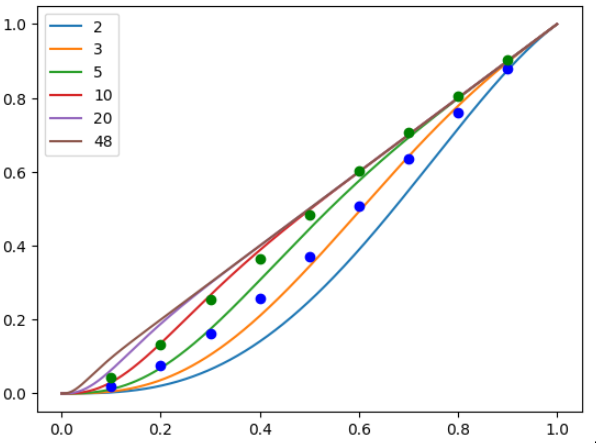
\includegraphics[width=1\textwidth,scale=0.5]{11-01-2023-23:03:16.png}
        Die grünen Punkt entschprechen der Messung bei einer Gruppengröße von k = 5, die blauen einer Gruppengröße von k = 2.

\end{document}

